\documentclass[hyperref=colorlinks]{beamer}
\mode<presentation>
\usetheme{iclpt}
\setbeamertemplate{navigation symbols}{}
\setbeamertemplate{headline}{
\begin{beamercolorbox}[leftskip=.2cm,rightskip=.2cm,topskip=.2cm,ht=1.1cm,dp=0.1cm,wd=\textwidth]{institute in head/foot}
  
\includegraphics[height=1cm]{icl.pdf}
  \hfill
  
\includegraphics[height=1cm]{../Pics/CMS-Color.pdf}
\end{beamercolorbox}
}
\setbeamertemplate{footline}{
\begin{beamercolorbox}[ht=.55cm,dp=0.4cm,wd=\textwidth,leftskip=.3cm]{author in head/foot}%
  \begin{minipage}[c]{5cm}%
    \usebeamerfont{author in head/foot}
    \insertshortauthor 
    \insertshorttitle
    \end{minipage}\hfill%
  \insertframenumber{} / \pageref{lastframe}
  \hfill
  \begin{minipage}{6cm}
    \hfill
  \end{minipage}
\end{beamercolorbox}%
}

\usepackage{color}
\usepackage{tabularx,colortbl}
\usepackage{graphicx}
\usepackage{pdfpages}
\usepackage{feynmp}
\DeclareGraphicsRule{*}{mps}{*}{}

\title{\vspace{-0.2cm} VBF Higgs to Invisible - Update}
\subtitle{HIG-14-038, AN-14-243\vspace{-0.7cm}}
\author[P. Dunne]{\underline{P. Dunne}} % A.M. Magnan and A. Nikitenko Joao Pela with \\ R. Aggleton, J. Brooke: Bristol \\ C.Asawangtrakuldee, Q.Li: Peking \\ P. Srimanobhas: Chulalongkorn \\ S. Kumar, K. Mazumdar: Mumbai}
\titlegraphic{
  \vspace{-0.7cm}
  %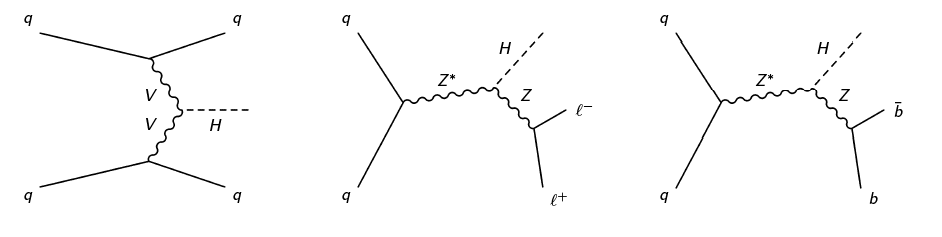
\includegraphics[width=\textwidth]{TalkPics/invcomb021213/feyndiags}
  %% \begin{fmfgraph*}(100,70)
  %%         \fmfleft{i1,i2}
  %%         \fmfright{o1,o2,o3}
  %%         \fmf{fermion}{i1,v1,o1}
  %%         \fmf{fermion}{i2,v2,o3}
  %%         \fmf{phantom,tension=4/5}{v1,v2}
  %%         \fmffreeze
  %%         \fmf{photon,label=$W,,Z$}{v1,v3}
  %%         \fmf{photon,label=$W,,Z$}{v2,v3}
  %%         \fmf{dashes}{v3,o2}
  %%         \fmflabel{$q$}{i1}
  %%         \fmflabel{$q$}{i2}
  %%         \fmflabel{$q$}{o1}
  %%         \fmflabel{$q$}{o3}
  %%         \fmflabel{$H$}{o2}
  %%       \end{fmfgraph*}
}
\date{}
\begin{document}
\begin{fmffile}{higgsexoupdatefeyndiags}

%TITLE PAGE
\section{Title}
\begin{frame}
  \titlepage
  
\end{frame}

\begin{frame}
  \frametitle{Overview}
  \begin{block}{}
    \scriptsize
    \begin{itemize}
    \item Preapproval conditions answered before Christmas
    \item Further study of single mu data suggested
    \item[-] Study variation of control region scale factors as cuts are varied
    \item[-] Use single mu data to study region below our trigger turn on
    \end{itemize}
  \end{block}
\end{frame}

\begin{frame}
  \frametitle{Study Procedure}
   \begin{block}{}
     \scriptsize
     \begin{itemize}
     \item Want to study source of $\frac{N_{Data}-N_{Bkg}}{N_{MC}}$ factors in control regions being $<1$
     \item[-] Hard to loosen several cuts due to trigger constraints
     \item[-] Use single mu trigger
     \item Study munu region:
     \item[-] Require 1 tight muon with $p_{T}>25$ GeV
     \item[-] Assume trigger fully efficient for jets
     \item Perform a grid search through variables we cut on:
     \item[-] jet 1 and 2 p$_{T}$, $M_{jj}$, jet-met min-dphi, met, met significance
     \item In following plots all cuts are as for the munu region unless stated otherwise:
     \item[-] jet 1 $p_{T}>50$ GeV, jet 2 p$_{T}>45$ GeV, $M_{jj}>1200$ GeV, jet-met min-dphi$>2.3$, met, met significance$>4$
     \end{itemize}
   \end{block}
  
\end{frame}

\begin{frame}
  \begin{block}{}
    \scriptsize
    \begin{itemize}
    \item met and jet 1 $p_{T}$ cuts have no discernable effect on scale factor:
    \item jet 2 $p_{T}$ and met significance have small effect: couple of percent
    \item Main effect from $M_{jj}$ and jet-met min-dphi
    \item[-] Plot shows scale factor as a function of the cut on these variables:
    \end{itemize}
    \vspace{-.6cm}

    \center
    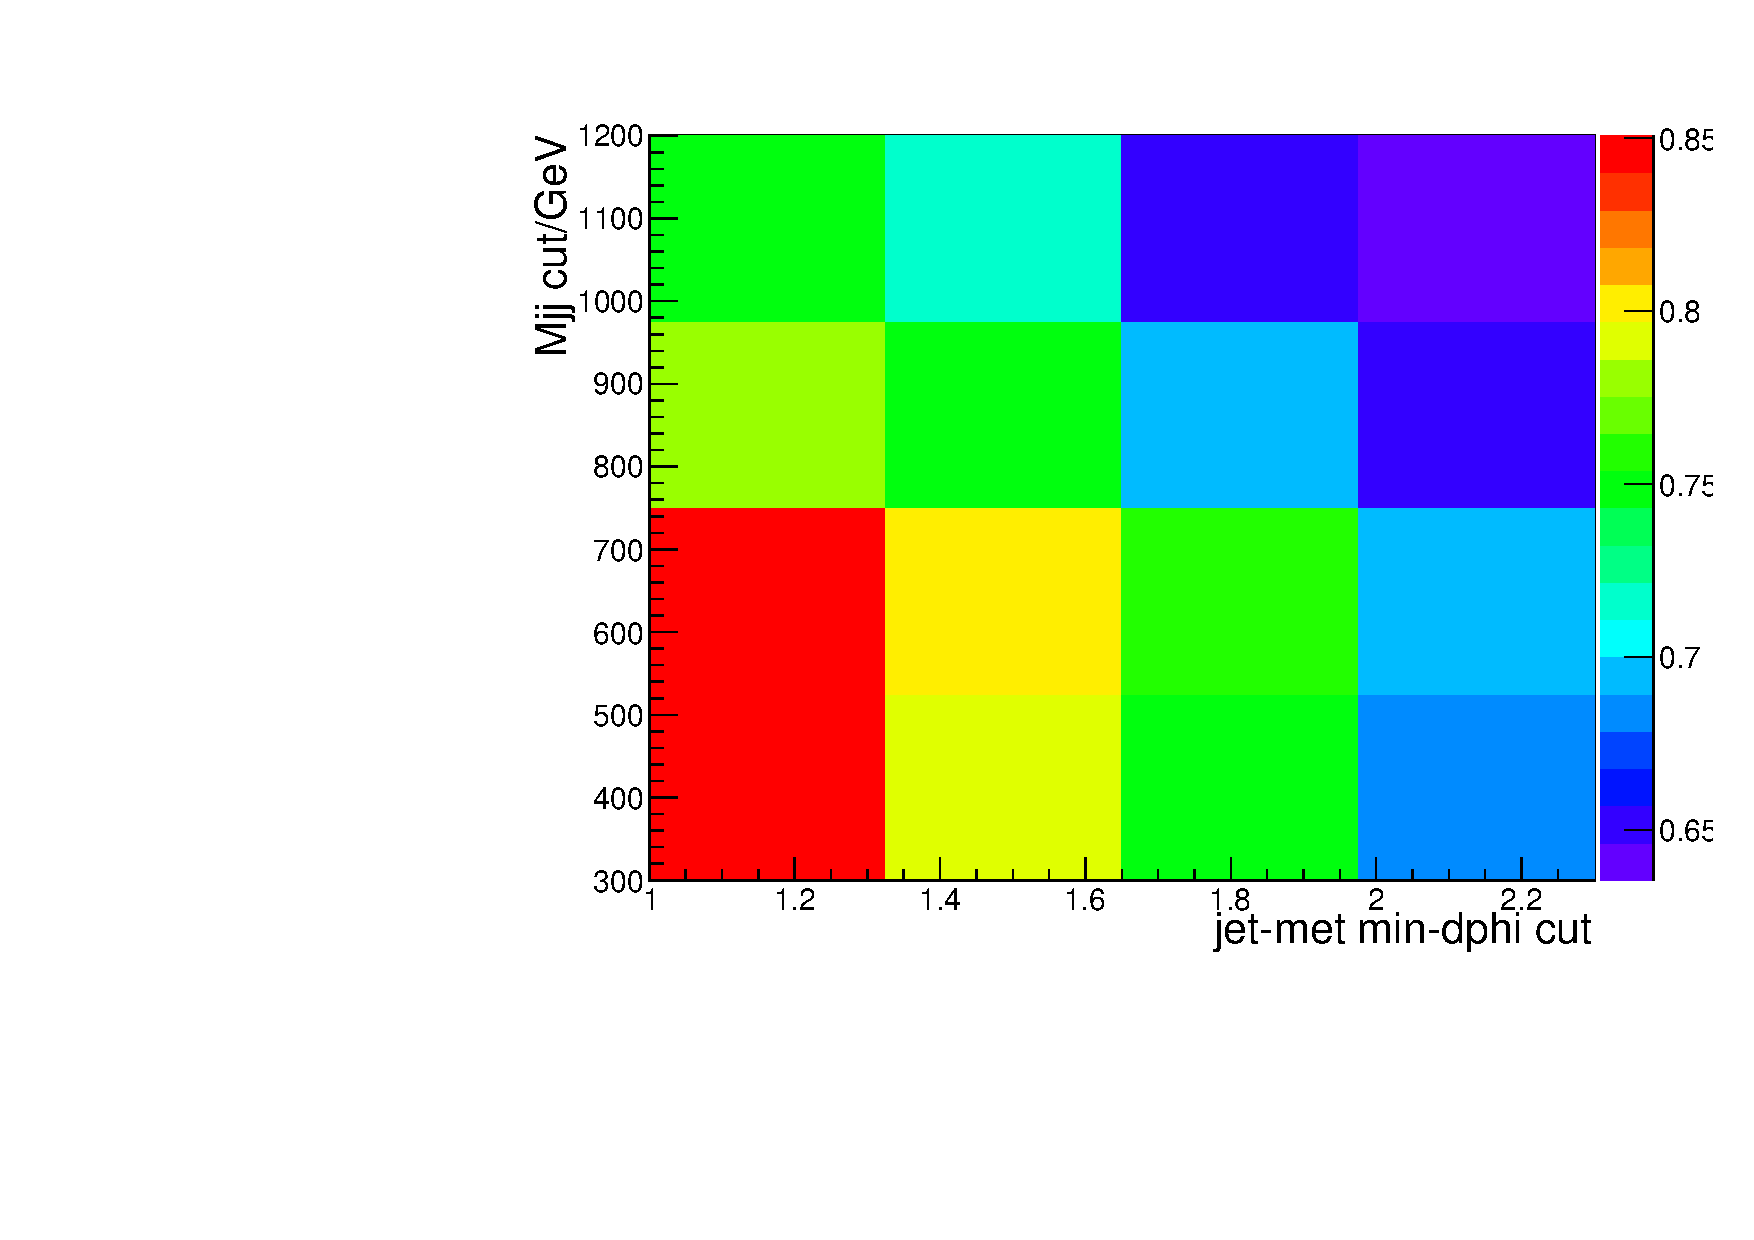
\includegraphics[width=.65\textwidth]{TalkPics/singlemustudy080115/jetmetdphimjj.pdf}
  \end{block}
\end{frame}

\begin{frame}
  \begin{block}{}
    \scriptsize
    \begin{itemize}
    \item Check whether it is only met phi causing scale factor variation
    \item Replace jet-met min-dphi cut with dijet dphi
    \item[-] nb dijet dphi is a less than cut so cut tightens with lower values
    \item Effect still seen and scale factor size is the same
    \end{itemize}
    \vspace{-.6cm}

    \center
    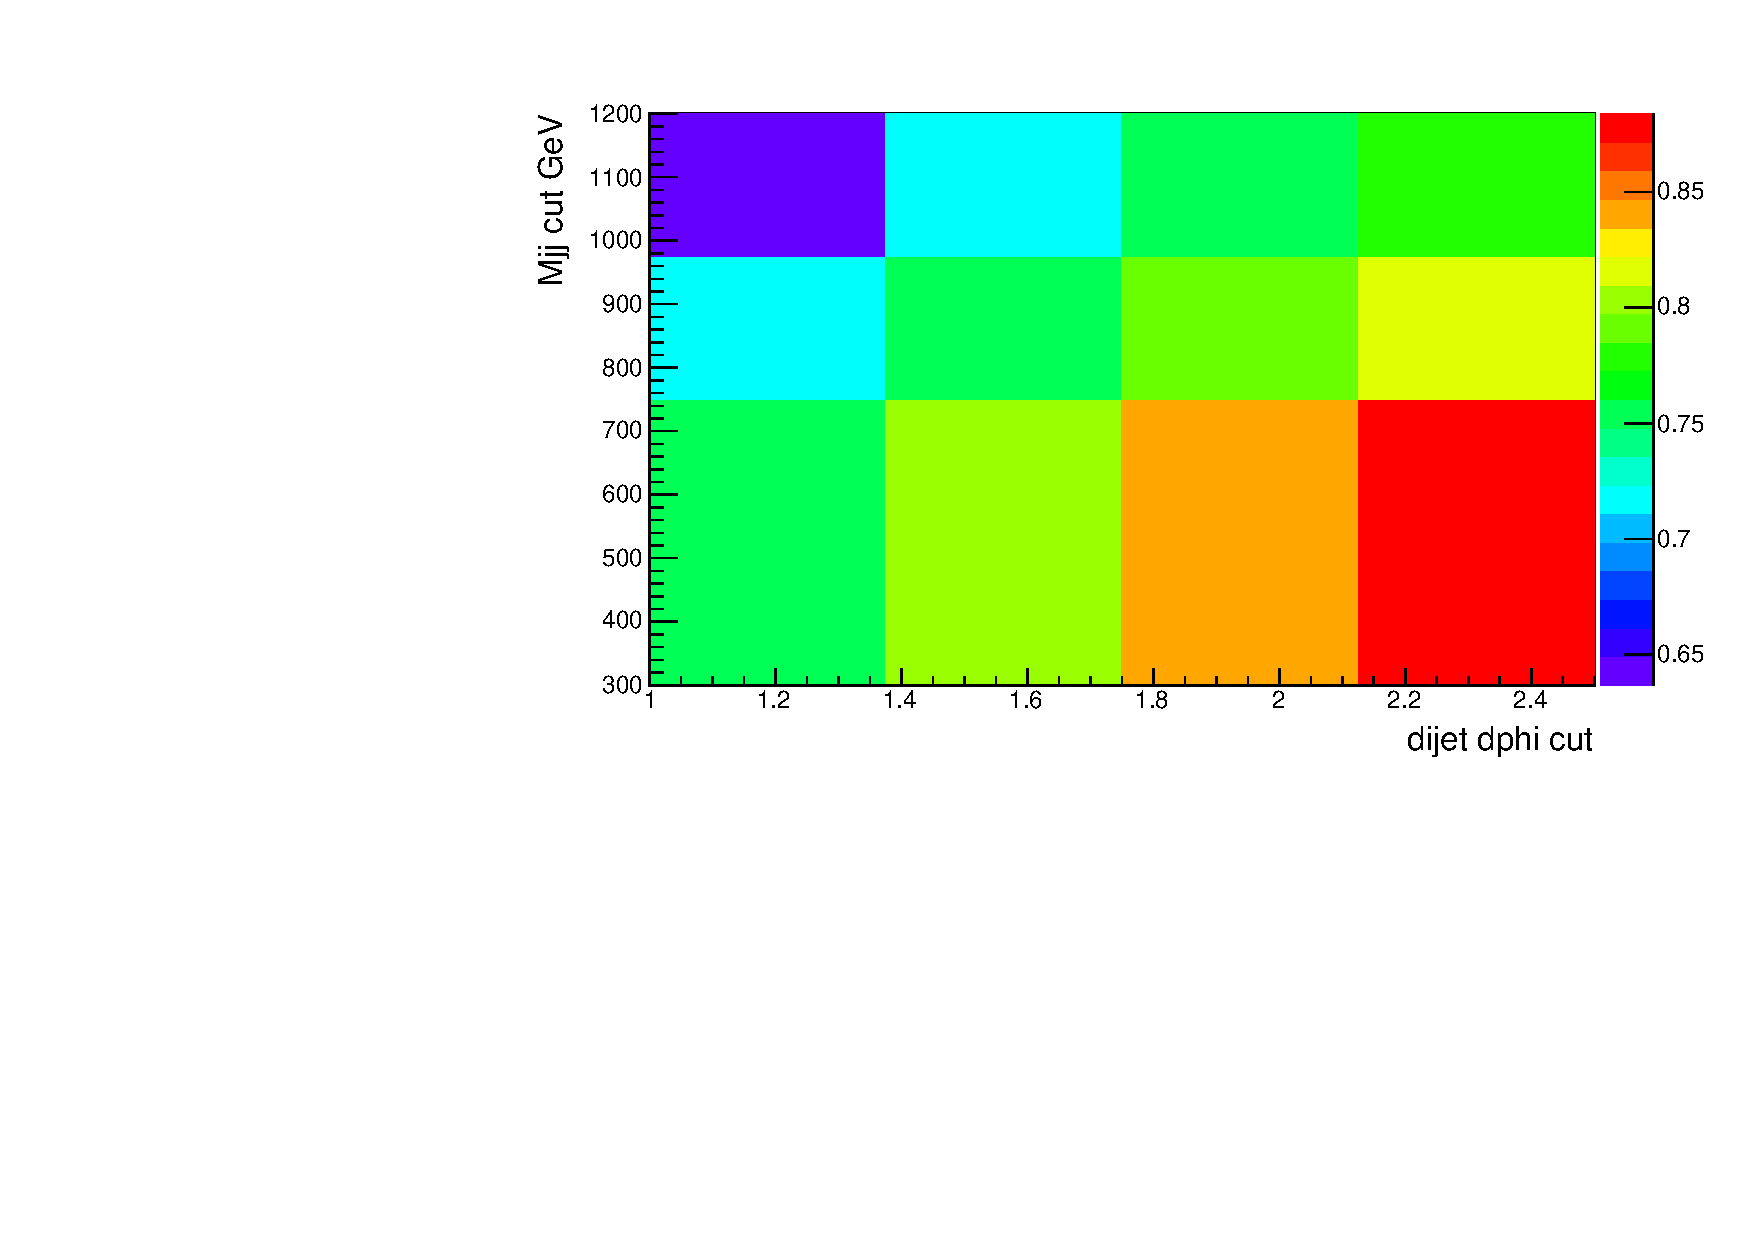
\includegraphics[width=.65\textwidth]{TalkPics/singlemustudy080115/dphijjmjj.pdf}
  \end{block}
\end{frame}

\begin{frame}
  \frametitle{Conclusion}
  \label{lastframe}
  \begin{block}{}
    \scriptsize
    \begin{itemize}
    \item $M_{jj}$ and jet-met min-dphi seem to be the main variables causing $<1$ scale factors
    \item Have swapped jet-met min-dphi for dijet dphi to see whether it is the jet or met phi which is most mismodelled
    \item[-] dijet dphi cut leads to same scale factor to jet-met min-dphi cut
    \item This suggests the issue is not made worse by using met phi
    \end{itemize}
    
  \end{block}

\end{frame}

\begin{frame}
  \frametitle{Backup}
\end{frame}

\end{fmffile}
\end{document}
